\documentclass[tikz,border=3mm,multi=tikzpicture]{standalone}
\usepackage[utf8]{inputenc}
\usepackage[T1]{fontenc}
\usepackage{helvet}
\renewcommand{\familydefault}{\sfdefault}
\usepackage{tikz}
\usetikzlibrary{angles,quotes,calc,intersections}

\begin{document}

\tikzset{every node/.append style={font=\sffamily\small}}

% TikZ 1 — Triângulo como polígono fechado
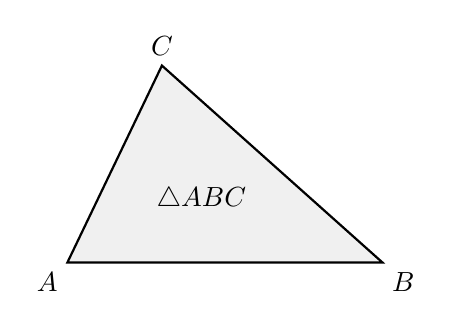
\begin{tikzpicture}[scale=1]
  \coordinate (A) at (0,0);
  \coordinate (B) at (4,0);
  \coordinate (C) at (1.2,2.5);

  \fill[gray!12] (A) -- (B) -- (C) -- cycle;
  \draw[thick] (A) -- (B) -- (C) -- cycle;

  \node[below left] at (A) {$A$};
  \node[below right] at (B) {$B$};
  \node[above] at (C) {$C$};
  \node at (1.7,0.8) {$\triangle ABC$};
\end{tikzpicture}

% TikZ 2 — Vértices e lados do triângulo ABC
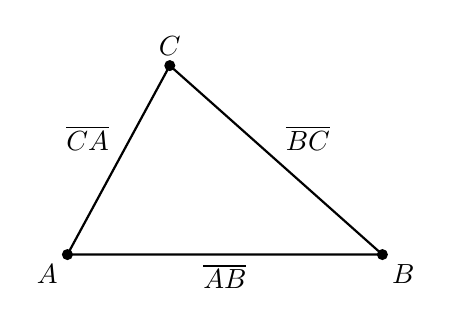
\begin{tikzpicture}[scale=1]
  \coordinate (A) at (0,0);
  \coordinate (B) at (4,0);
  \coordinate (C) at (1.3,2.4);

  \draw[thick] (A) -- (B) -- (C) -- cycle;
  \fill (A) circle (2pt);
  \fill (B) circle (2pt);
  \fill (C) circle (2pt);

  \node[below left] at (A) {$A$};
  \node[below right] at (B) {$B$};
  \node[above] at (C) {$C$};
  \node[below] at ($(A)!0.5!(B)$) {$\overline{AB}$};
  \node[above right] at ($(B)!0.5!(C)$) {$\overline{BC}$};
  \node[above left] at ($(C)!0.5!(A)$) {$\overline{CA}$};
\end{tikzpicture}

% TikZ 3 — Ângulos internos do triângulo ABC
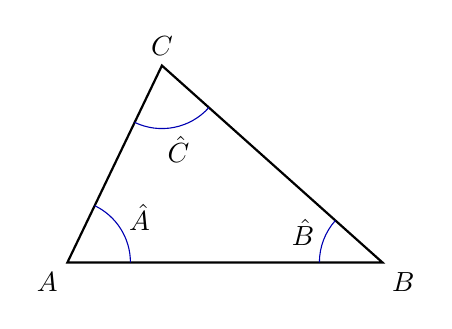
\begin{tikzpicture}[scale=1]
  \coordinate (A) at (0,0);
  \coordinate (B) at (4,0);
  \coordinate (C) at (1.2,2.5);

  \draw[thick] (A) -- (B) -- (C) -- cycle;
  \pic[draw=blue!70!black, "$\hat{A}$", angle radius=8mm, angle eccentricity=1.35] {angle = B--A--C};
  \pic[draw=blue!70!black, "$\hat{B}$", angle radius=8mm, angle eccentricity=1.35] {angle = C--B--A};
  \pic[draw=blue!70!black, "$\hat{C}$", angle radius=8mm, angle eccentricity=1.35] {angle = A--C--B};

  \node[below left] at (A) {$A$};
  \node[below right] at (B) {$B$};
  \node[above] at (C) {$C$};
\end{tikzpicture}

% TikZ 4 — Altura relativa ao lado AB
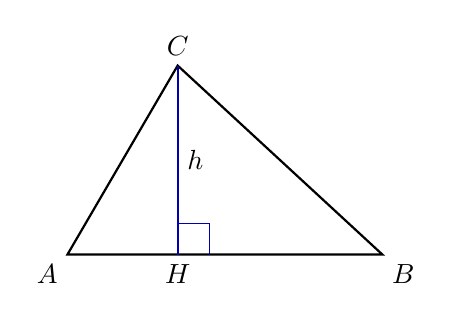
\begin{tikzpicture}[scale=1]
  \coordinate (A) at (0,0);
  \coordinate (B) at (4,0);
  \coordinate (C) at (1.4,2.4);
  \coordinate (H) at (1.4,0);

  \draw[thick] (A) -- (B) -- (C) -- cycle;
  \draw[blue!70!black, thick] (C) -- (H);
  \pic[draw=blue!70!black, angle radius=4mm] {right angle = C--H--B};

  \node[below left] at (A) {$A$};
  \node[below right] at (B) {$B$};
  \node[above] at (C) {$C$};
  \node[below] at (H) {$H$};
  \node[right] at ($(C)!0.5!(H)$) {$h$};
\end{tikzpicture}

% TikZ 5 — Mediana relativa ao lado AB
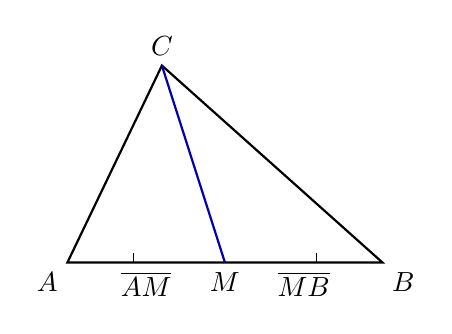
\begin{tikzpicture}[scale=1]
  \coordinate (A) at (0,0);
  \coordinate (B) at (4,0);
  \coordinate (C) at (1.2,2.5);
  \coordinate (M) at ($(A)!0.5!(B)$);

  \draw[thick] (A) -- (B) -- (C) -- cycle;
  \draw[blue!70!black, thick] (C) -- (M);
  \draw ($(A)!0.42!(M)$) -- ++(0,0.12);
  \draw ($(M)!0.58!(B)$) -- ++(0,0.12);

  \node[below left] at (A) {$A$};
  \node[below right] at (B) {$B$};
  \node[above] at (C) {$C$};
  \node[below] at (M) {$M$};
  \node[below] at ($(A)!0.5!(M)$) {$\overline{AM}$};
  \node[below] at ($(M)!0.5!(B)$) {$\overline{MB}$};
\end{tikzpicture}

% TikZ 6 — Bissetriz do ângulo A
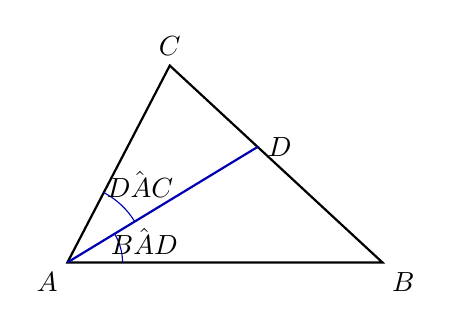
\begin{tikzpicture}[scale=1]
  \coordinate (A) at (0,0);
  \coordinate (B) at (4,0);
  \coordinate (C) at (1.3,2.5);
  \coordinate (D) at (2.42,1.47);

  \draw[thick] (A) -- (B) -- (C) -- cycle;
  \draw[blue!70!black, thick] (A) -- (D);
  \pic[draw=blue!70!black, "$\hat{BAD}$", angle radius=7mm, angle eccentricity=1.45] {angle = B--A--D};
  \pic[draw=blue!70!black, "$\hat{DAC}$", angle radius=10mm, angle eccentricity=1.35] {angle = D--A--C};

  \node[below left] at (A) {$A$};
  \node[below right] at (B) {$B$};
  \node[above] at (C) {$C$};
  \node[right] at (D) {$D$};
\end{tikzpicture}

\end{document}
